\documentclass[conference]{IEEEtran}
% \IEEEoverridecommandlockouts
% The preceding line is only needed to identify funding in the first footnote. If that is unneeded, please comment it out.
\usepackage{cite}
\usepackage{amsmath,amssymb,amsfonts}
\usepackage{graphicx}
\usepackage{textcomp}
\usepackage{xcolor}
\usepackage{booktabs}
\usepackage{tabularx}
\usepackage{makecell}
\usepackage{url}
\usepackage{tikz}
\usetikzlibrary{shapes.geometric, arrows.meta, positioning}
\usepackage{pgfplots}
\pgfplotsset{compat=1.18}
% Categorical chart palette (validated: CVD-safe adjacent pairs on a light surface).
\definecolor{vizblue}{HTML}{2A78D6}
\definecolor{vizorange}{HTML}{EB6834}
\def\BibTeX{{\rm B\kern-.05em{\sc i\kern-.025em b}\kern-.08em
    T\kern-.1667em\lower.7ex\hbox{E}\kern-.125emX}}
\begin{document}
\raggedbottom

\title{Speech-Native Retrieval-Augmented Generation for Agricultural Advisory in Low-Resource Dialects}
% \thanks{Identify applicable funding agency here. If none, delete this.}

\author{\IEEEauthorblockN{Darshan Pundlik Heble}
\IEEEauthorblockA{\textit{PG Scholar, Department of Computer Science} \\
\textit{Christ (Deemed to be University)}\\
Bangalore, India \\
darshanpundlik.heble@mca.christuniversity.in }
\and
\IEEEauthorblockN{Newbegin M}
\IEEEauthorblockA{\textit{Department of Computer Science} \\
\textit{Christ (Deemed to be University)}\\
Bangalore, India \\
new.begin@christuniversity.in}
\and
\IEEEauthorblockN{Benita Jose Chalissery}
\IEEEauthorblockA{\textit{Department of Computer Science} \\
\textit{Christ (Deemed to be University)}\\
Bangalore, India \\
benita.jaison@christuniversity.in}
}

\maketitle

\begin{abstract}
Smallholder farmers in low-literacy, dialect-rich regions are typically served by voice-enabled advisory systems that first transcribe a spoken query via automatic speech recognition (ASR) before retrieval-augmented generation (RAG) produces an answer. Because domain-critical terminology (pesticide, disease, and pest names) is disproportionately subject to ASR substitution errors, and this worsens under dialectal and colloquial variation, transcription errors propagate directly into retrieval failures and incorrect advice. Retrieving directly from speech embeddings removes this failure mode, but no existing system combines speech-native retrieval with an explicit dialect-to-scientific-entity mapping layer, confidence-gated escalation to a human expert, and fully offline operation on consumer hardware. This paper proposes a framework integrating these four components and an experimental protocol comparing ASR-cascaded, keyword, dense, and hybrid retrieval under dialect variation. A runnable prototype was built and measured on demo-scale data: on ground-truth query text, dialect mapping is what makes dialectal queries retrievable at all (recall@1 rising from 0.000 to 0.615), and per-stage latency fits comfortably within a 6~GB-VRAM budget in fp16; on synthesized speech audio, neither the ASR-cascaded nor the speech-native condition approaches text-input retrieval. Retraining the speech-native adapter with dialect-lexicon-normalized distillation targets (embedding-space dialect mapping, with no transcript at inference) lifts its recall@1 from chance (0.020) to 0.127 and its dialectal recall@1 above the ASR cascade's (0.141 vs.\ 0.038), leaving the central speech-native premise unconfirmed but directionally supported, pending real target-dialect speech, which does not yet exist. Follow-up measurements show the confidence gate's apparent open-book-signal weakness was an artifact of its first validation set rather than a design flaw, and that INT8/INT4 quantization unexpectedly \emph{increases} per-query latency several-fold on this GPU despite reducing memory use.
\end{abstract}

\renewcommand\IEEEkeywordsname{Keywords}
\begin{IEEEkeywords}
Agricultural advisory systems, dialect-aware retrieval, low-resource languages, speech-native RAG.
\end{IEEEkeywords}

\section{Introduction}
Agricultural extension, the transfer of evidence-based farming knowledge to smallholder farmers, remains a critical bottleneck in regions with low literacy and limited connectivity. RAG-based advisory systems such as Farmer.Chat \cite{farmerchat2024} and KrishokBondhu \cite{ameen2026krishokbondhu} show that voice-enabled, multilingual chatbots can reduce farmers' dependence on scarce extension agents, and systems such as SukhaRakshak AI \cite{iwmi2025sukharakshak} extend this to more than twenty Indian languages. All of them, however, first transcribe a spoken query via ASR before retrieval proceeds on the resulting text. ASR errors on Indian-language agricultural speech disproportionately affect domain-critical terms \cite{benchmarkingasr2026}, and this degrades further under dialectal and code-mixed variation \cite{dialectmatters2026}; a mistranscribed pest or disease term propagates directly into retrieval, and ultimately into an incorrect recommendation.

Retrieving directly from a speech representation removes this failure mode. Amazon's SpeechRAG \cite{min2025speechrag} aligns a speech encoder with a frozen text-retrieval embedding space, and Google's Speech-to-Retrieval (S2R) \cite{google2025s2r} performs an analogous mapping live in production. Neither, however, has been evaluated under dialect variation or domain-critical rare-entity retrieval, and neither normalizes the regional or colloquial terms a farmer may use for the same concept; existing agricultural knowledge graphs \cite{wu2026cropgraphrag,kgeditorial2023} normalize only standardized, written terminology. A further limitation is that existing systems answer regardless of confidence, even though incorrect advice can damage a season's crop, an argument made explicitly for comparably high-stakes RAG deployments in clinical and financial domains \cite{dependablerag2026,abstinence2025}, though naive confidence signals are known to misfire in both directions \cite{intrygue2026}. Most RAG research also implicitly assumes reliable connectivity and cloud-hosted inference \cite{compactllm2026}, which the rural settings targeted here frequently lack. No existing system combines speech-native retrieval, dialect-to-entity mapping, confidence-gated escalation, and offline operation for agricultural advisory in low-resource dialects. This paper poses:

\begin{itemize}
    \item \textbf{RQ1:} Does speech-native retrieval retain its advantage over ASR-cascaded retrieval under dialect variation and domain-critical rare vocabulary?
    \item \textbf{RQ2:} Does a dialect-to-scientific-entity mapping layer improve retrieval accuracy for regional or colloquial phrasing?
    \item \textbf{RQ3:} Can the pipeline operate fully offline, on consumer hardware, at acceptable latency and accuracy?
    \item \textbf{RQ4:} Does hybrid (lexical + dense) retrieval with dialect mapping outperform either method alone on domain-critical rare entities?
\end{itemize}

\noindent The main contributions are: (1) identifying dialect variation combined with domain-critical rare vocabulary as an underaddressed gap in speech-native retrieval \cite{min2025speechrag,google2025s2r}; (2) a dialect-to-scientific-entity mapping layer bootstrapped from low-cost public resources rather than new dialect speech collection; (3) a confidence-gated architecture that escalates low-confidence queries to a human expert; and (4) a system design scoped to consumer-grade, GPU-constrained hardware, reserving cloud GPU resources only for one-time adapter training.

Section II reviews related work; Section III presents the proposed architecture; Section IV describes the experimental protocol and reports real, measured preliminary results from a runnable prototype on demo-scale data; Section V concludes.

\section{Related Work}

A growing body of work applies RAG to agricultural advisory. Farmer.Chat \cite{farmerchat2024} is deployed across four countries with multilingual, multimodal input; KrishokBondhu \cite{ameen2026krishokbondhu} is architecturally closest to the present proposal, a phone-call-based voice-in/voice-out pipeline for Bengali farmers that outperformed the KisanQRS benchmark \cite{rehman2023kisanqrs} by 44.7\% on a composite quality score; SukhaRakshak AI \cite{iwmi2025sukharakshak}, AgroLLM \cite{agrollm2025}, and a multi-LLM evaluation framework \cite{sawant2026farmeraiframework} extend or benchmark this pattern further. A.A.H.A.R. \cite{dubey2025aahar} combines an offline, quantized LLM with an ASR component fine-tuned for agricultural vocabulary and accents, and Krishi Sathi \cite{vijayvargia2025krishisathi} is an intent-aware bilingual QA chatbot with 97.53\% reported accuracy, but both remain ASR-then-retrieval cascades that adapt only the ASR component to dialect. A Bengali cross-lingual case study \cite{hossain2026bengalirag} already bridges colloquial and scientific terminology via keyword injection, and explicitly names ASR integration and dialect-aware normalization of spoken queries as its own unaddressed future work. None of these systems treats ASR-induced retrieval failure on dialect-specific or domain-critical terminology as a first-class design problem to be solved by restructuring retrieval rather than by adapting ASR alone.

Benchmarking work on Indian-language agricultural ASR \cite{benchmarkingasr2026} shows that standard word-error-rate metrics under-penalize errors on crop, chemical, and pest vocabulary specifically, and a complementary study on cross-lingual transfer \cite{dialectmatters2026} quantifies how code-mixing degrades transcription for dialects with no dedicated resource. Dedicated corpora exist for some varieties, such as a 250-hour Chhattisgarhi dataset \cite{singh2023respin}, but remain incomplete in coverage. Speech-native retrieval itself (SpeechRAG \cite{min2025speechrag} and S2R \cite{google2025s2r}, built on self-supervised speech encoders such as wav2vec~2.0 \cite{baevski2020wav2vec} and HuBERT \cite{hsu2021hubert}, the ``textless NLP'' literature \cite{spidr2025}, and multilingual encoders such as SeamlessM4T \cite{barrault2023seamlessm4t}) has not been evaluated under dialect variation or domain-critical rare-entity retrieval, and neither targets agriculture.

Comparative retrieval studies \cite{sultania2024hybridsearch} find dense retrieval stronger on paraphrased queries and lexical methods stronger on exact, rare, domain-specific entities, motivating hybrid fusion over either alone. Colloquial-to-formal mapping is shown to be necessary and tractable in text by a soft-prompt-tuning approach over agricultural knowledge graphs \cite{liu2025colloquialpest,wu2026cropgraphrag,yao2024agcner,kgeditorial2023} and by the keyword-injection strategy above \cite{hossain2026bengalirag}, but neither operates on speech. Confidence-gated abstention is argued for high-stakes RAG in clinical and financial domains \cite{dependablerag2026,abstinence2025}, but naive entropy-based signals are shown to misfire in both directions \cite{intrygue2026}, requiring empirical validation rather than blind trust. On-device deployment is bounded by reported figures for quantized LLMs (2--3 tokens/second for 4-bit Llama-3~8B on 6~GB-RAM smartphones) \cite{compactllm2026}; A.A.H.A.R. and the Bengali case study \cite{dubey2025aahar,hossain2026bengalirag} already demonstrate fully local text-based agricultural RAG, and a vision-modality offline system in rural Tigray \cite{tigray2025plantdisease} demonstrates the same deployment pattern for a different modality.

Taken together, no system located during this review combines speech-native retrieval, dialect-aware mapping, confidence-gated escalation, and offline operation, and one of the closest text-based systems in the same problem space explicitly names this combination as unaddressed future work of its own \cite{hossain2026bengalirag}.

\section{Proposed Architecture}

\subsection{Design Overview}
The architecture integrates the four components motivated in Section I into a single pipeline (Fig.~\ref{fig:architecture}). A spoken query is mapped directly into a retrieval-ready representation without an intervening transcription step (\S III-B); the result is normalized against a dialect-to-scientific-entity mapping layer (\S III-C); retrieval is performed by a hybrid lexical-dense retriever (\S III-D); the retrieved evidence and a confidence score pass through a gate that either proceeds to generation or escalates to a human expert (\S III-E); and every stage except one-time adapter training runs fully offline on consumer-grade hardware (\S III-F).

\begin{figure}[t]
\centering
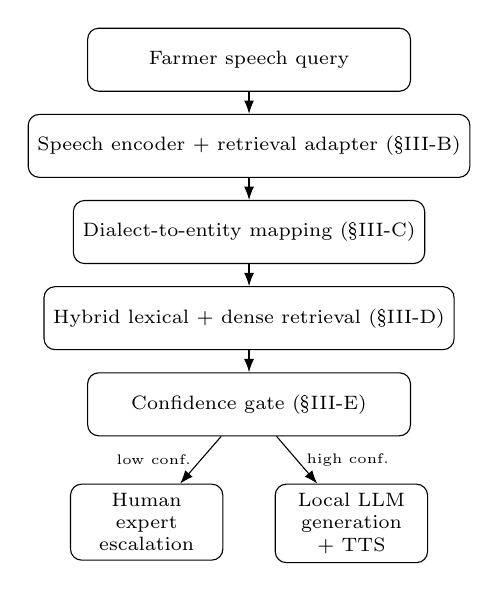
\begin{tikzpicture}[
  block/.style={rectangle, draw, rounded corners, align=center, minimum width=4.1cm, minimum height=0.8cm, font=\scriptsize},
  smallblock/.style={rectangle, draw, rounded corners, align=center, text width=1.7cm, font=\scriptsize},
  arr/.style={-Latex}
]
\node[block] (speech) {Farmer speech query};
\node[block, below=0.28cm of speech] (enc) {Speech encoder + retrieval adapter (\S III-B)};
\node[block, below=0.28cm of enc] (dial) {Dialect-to-entity mapping (\S III-C)};
\node[block, below=0.28cm of dial] (hyb) {Hybrid lexical + dense retrieval (\S III-D)};
\node[block, below=0.28cm of hyb] (conf) {Confidence gate (\S III-E)};
\node[smallblock, below=0.6cm of conf, xshift=-1.3cm] (esc) {Human expert escalation};
\node[smallblock, below=0.6cm of conf, xshift=1.3cm] (gen) {Local LLM generation + TTS};

\draw[arr] (speech) -- (enc);
\draw[arr] (enc) -- (dial);
\draw[arr] (dial) -- (hyb);
\draw[arr] (hyb) -- (conf);
\draw[arr] (conf) -- node[left,font=\tiny]{low conf.} (esc);
\draw[arr] (conf) -- node[right,font=\tiny]{high conf.} (gen);
\end{tikzpicture}
\caption{Proposed pipeline. All stages except one-time adapter training (\S III-F) run fully offline on consumer-grade hardware.}
\label{fig:architecture}
\end{figure}

\subsection{Speech-Native Retrieval Backbone}
Following SpeechRAG \cite{min2025speechrag} and S2R \cite{google2025s2r}, the pipeline fine-tunes a lightweight adapter projecting representations from a pretrained speech encoder (wav2vec~2.0 \cite{baevski2020wav2vec}, HuBERT \cite{hsu2021hubert}, or SeamlessM4T \cite{barrault2023seamlessm4t} where the target dialect lacks dedicated pretraining data) into the embedding space of a frozen text retriever, extending dense passage retrieval \cite{karpukhin2020dpr} to speech queries. This adapter is the only component permitted cloud GPU use, and only once, at training time; at inference it runs locally. Unlike prior SpeechRAG/S2R evaluations, it is trained and evaluated with explicit attention to domain-critical rare entities and dialectal or code-mixed phrasing, since both independently degrade ASR accuracy \cite{benchmarkingasr2026,dialectmatters2026} and are expected to compound.

\subsection{Dialect-to-Scientific-Entity Mapping Layer}
The mapping layer bootstraps a dialect-term-to-scientific-entity lexicon from existing public resources (agricultural knowledge graphs \cite{wu2026cropgraphrag}, named-entity resources \cite{yao2024agcner}, and standards-level ontologies \cite{kgeditorial2023}) rather than new dialect speech collection, following the motivation of \cite{liu2025colloquialpest,hossain2026bengalirag}, both of which operate on written text where this system operates on the speech-embedding representation of \S III-B. A post-ASR text-normalization path is retained only as a fallback, since it reintroduces a transcription dependency; an embedding-space mapping path that aligns dialect-term speech embeddings directly against the retriever's embedding space is preferred.

\subsection{Hybrid Retrieval Strategy}
Dense retrieval outperforms lexical retrieval on paraphrased, low-lexical-overlap queries, while lexical methods retain the advantage on exact, rare, domain-specific entities \cite{sultania2024hybridsearch}: precisely the pesticide and disease category this paper treats as safety-critical. The architecture therefore fuses lexical and dense signals rather than committing to either alone, deliberately against a naive ``speech embeddings beat keywords'' framing that would risk losing this safety-critical category to a simpler baseline.

\subsection{Confidence-Gated Escalation}
Because an incorrect recommendation can damage a season's crop, a confidence gate sits between retrieval and generation, following the case for confidence-gated abstention in comparably high-stakes RAG deployments \cite{abstinence2025}. It combines closed-book (internal model confidence) and open-book (context-conditioned divergence) signals, per the taxonomy of \cite{dependablerag2026}, since naive single-signal confidence estimates are known to misfire in both directions \cite{intrygue2026}; accordingly it is treated as requiring empirical validation (\S IV-A) rather than assumed reliable by construction. Below-threshold queries escalate to a human expert, mirroring the human-in-the-loop fallback in KrishokBondhu \cite{ameen2026krishokbondhu}.

\subsection{Offline Deployment Scoping}
All stages other than one-time adapter training run without a live network connection on consumer-grade, GPU-constrained hardware, mirroring the deployment pattern of text-only offline agricultural RAG \cite{dubey2025aahar,hossain2026bengalirag} and a vision-modality offline system \cite{tigray2025plantdisease}, bounded by reported feasibility figures for quantized on-device LLMs \cite{compactllm2026}. Whether these figures hold once a speech encoder, adapter, dialect-mapping layer, and confidence gate are stacked on top of generation is RQ3, evaluated next.

\section{Experimental Evaluation}

\subsection{Protocol and Metrics}
No experiments on the target dialect have yet been executed on the protocol below; a runnable prototype's preliminary results follow in \S IV-C. The evaluation requires a query set stratified along two axes: standard-terminology versus dialectal/colloquial phrasing, and common versus domain-critical rare-entity queries, informed by prior characterizations of real farmer helpline query content \cite{godara2022querycount,godara2020sequentialpattern}. Where dedicated dialect speech resources exist, such as the RESPIN Chhattisgarhi corpus \cite{singh2023respin}, they are used directly; otherwise a small evaluation set is collected for the rare-entity and dialectal strata, consistent with collecting no large new dialect speech corpus for training. Four retrieval conditions are compared: ASR-cascaded (Whisper \cite{radford2023whisper} transcription then text retrieval, the dominant existing pattern), keyword-only (BM25), dense semantic \cite{karpukhin2020dpr}, and hybrid, each evaluated with and without dialect mapping to isolate its contribution. Retrieval quality is measured via recall@$k$ and MRR, reported per stratum rather than aggregated, following the rationale behind the agriculture-weighted WER metric of \cite{benchmarkingasr2026}. The confidence gate is validated on a held-out labeled set, scoring closed- and open-book signals \cite{dependablerag2026} against ground-truth correctness before being credited with any end-to-end result \cite{intrygue2026}, and all inference-time components are benchmarked on one explicitly stated consumer-hardware configuration.

\subsection{Evaluation Hypotheses}
For RQ1, speech-native retrieval is hypothesized to match or exceed ASR-cascaded retrieval in aggregate, with the gap \emph{growing} on dialectal/rare-entity strata, where ASR error concentrates \cite{benchmarkingasr2026,dialectmatters2026}; a shrinking or reversed gap there would indicate the adapter fails to generalize to dialect variation. For RQ2, dialect mapping is hypothesized to improve accuracy specifically on the dialectal stratum, with little change on standard phrasing; a uniform gain across both would indicate a general rather than dialect-targeted effect. For RQ3, the full pipeline is hypothesized to meet a pre-specified latency budget on the stated hardware without material accuracy loss; exceeding the budget or a substantial accuracy regression under quantization would answer RQ3 negatively. For RQ4, hybrid retrieval with mapping is hypothesized to outperform lexical-only and dense-only retrieval individually on the rare-entity stratum \cite{sultania2024hybridsearch}; parity with either alone would indicate the fusion adds complexity without benefit.

\subsection{Prototype and Preliminary Results}
A best-effort, runnable prototype of Fig.~\ref{fig:architecture} was built and measured end to end on small, hand-curated, demo-scale data (not the dialect-stratified corpus \S IV-A calls for) and, because no recorded speech corpus for the target dialect exists, every audio measurement below uses \texttt{espeak-ng} text-to-speech synthesis rather than native dialect speech. These results are therefore an engineering stress-test of the mechanism, not an answer to RQ1--RQ4 as posed. The prototype combines a hybrid BM25 + dense retriever (Reciprocal Rank Fusion, $k{=}60$) over a 42-passage knowledge base, a 29-entry dialect lexicon, a speech-native adapter over frozen wav2vec2 hidden states \cite{baevski2020wav2vec,min2025speechrag,google2025s2r} trained to distill the text retriever's sentence embeddings, an ASR-cascaded baseline using \texttt{faster-whisper} ``tiny'' \cite{radford2023whisper}, and a confidence gate per \cite{dependablerag2026}, with Qwen2.5-0.5B-Instruct (fp16) generation. All measurements ran on one NVIDIA RTX~3050 Laptop GPU (6~GB VRAM) over 50 queries stratified 2$\times$2 over standard/dialectal phrasing and common/rare entities.

Table~\ref{tab:retrieval} reports recall@1 for six conditions; Fig.~\ref{fig:retrieval-chart} visualizes the standard-vs.-dialectal split for the four text-input conditions. Dialect mapping is the single largest lever measured: every text-input condition without it scores at or near zero on both dialectal strata, while adding it raises dialectal recall@1 to 0.615: a demo-scale confirmation of the RQ2/RQ4 premise. The ASR-cascaded baseline is badly degraded on dialectal queries (0.038 recall@1) and underperforms text-only hybrid retrieval even on standard phrasing, consistent with the ASR-error concentration reported by \cite{benchmarkingasr2026,dialectmatters2026}. A first speech-native adapter, trained on 108 short English templates aligned to passage embeddings, reached 61.1\% on its own template validation split but only 0.020 recall@1 (chance) on the evaluation set: it memorized phrasing rather than learning to retrieve. Retraining it on KB passage sentences, entity-alias templates, and romanized-Hindi lexicon-term templates (three TTS voice/speed variants), to reproduce the text embedding of each utterance's \emph{own} sentence \cite{min2025speechrag}, raises held-out recall@1 to 0.127 (three-seed mean). For dialectal utterances the target is the embedding of the \emph{lexicon-normalized} sentence, giving the embedding-space dialect-mapping path of \S III-C with no transcript at inference. An ablation with raw dialectal targets drops mean dialectal recall@1 from 0.141 to 0.038 (normalization wins for every seed) at some cost on standard phrasing (0.111 vs.\ 0.194). With 26 dialectal queries on synthetic audio this is a directional signal for RQ1, not a confirmation.

\begin{table}[t]
\caption{Recall@1 by retrieval condition and query stratum (prototype, $n{=}50$). Conditions 1--4 take ground-truth text; only 5--6 take synthesized speech audio. $^\dagger$Mean of three training seeds.}
\centering
\footnotesize
\begin{tabular}{@{}lccc@{}}
\toprule
\textbf{Condition} & \textbf{All} & \textbf{Std.} & \textbf{Dial.} \\
\midrule
1. Keyword only (BM25) [text]           & 0.500 & 0.958 & 0.077 \\
2. Dense only [text]                    & 0.400 & 0.833 & 0.000 \\
3. Hybrid, no dialect map. [text]       & 0.460 & 0.958 & 0.000 \\
4. Hybrid + dialect map. [text]         & \textbf{0.780} & 0.958 & \textbf{0.615} \\
5. ASR cascade + hybrid + map. [audio]  & 0.400 & 0.792 & 0.038 \\
6. Speech-native, emb. map. [audio]$^\dagger$ & 0.127 & 0.111 & 0.141 \\
\quad 6a. raw dialect targets$^\dagger$       & 0.113 & 0.194 & 0.038 \\
\quad 6b. first-version adapter          & 0.020 & 0.000 & 0.038 \\
\bottomrule
\end{tabular}
\label{tab:retrieval}
\end{table}

\begin{figure}[t]
\centering
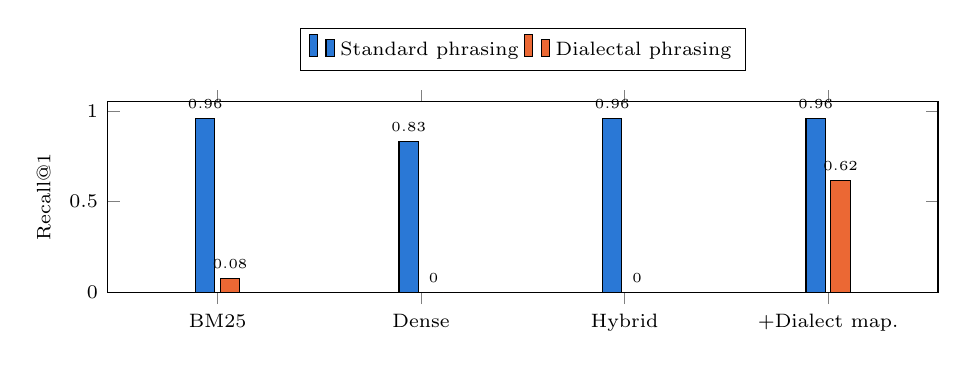
\begin{tikzpicture}
\begin{axis}[
  ybar,
  bar width=7pt,
  width=\columnwidth,
  height=4cm,
  ymin=0, ymax=1.05,
  ylabel={Recall@1},
  symbolic x coords={bm25,dense,hybrid,hybriddm},
  xtick=data,
  xticklabels={BM25,Dense,Hybrid,{+Dialect map.}},
  x tick label style={font=\scriptsize},
  y tick label style={font=\scriptsize},
  ylabel style={font=\scriptsize},
  legend style={font=\scriptsize, at={(0.5,1.16)}, anchor=south, legend columns=-1},
  enlarge x limits=0.18,
  nodes near coords,
  nodes near coords style={font=\tiny},
  every node near coord/.append style={/pgf/number format/.cd, fixed, precision=2},
]
\addplot[fill=vizblue, draw=black] coordinates {(bm25,0.9585) (dense,0.833) (hybrid,0.9585) (hybriddm,0.9585)};
\addplot[fill=vizorange, draw=black] coordinates {(bm25,0.077) (dense,0.000) (hybrid,0.000) (hybriddm,0.615)};
\legend{Standard phrasing, Dialectal phrasing}
\end{axis}
\end{tikzpicture}
\caption{Recall@1 for standard- vs.\ dialectal-phrasing queries, averaged over common/rare strata (text-input conditions 1--4). Dialect mapping is the only lever tested that lifts dialectal recall above near-zero.}
\label{fig:retrieval-chart}
\end{figure}

The confidence gate was first validated on 50 templated-answer examples (0.780 unconditional accuracy); at its best threshold it answered 32\% of queries at 0.875 accuracy while escalating 81.8\% of wrong answers, but its open-book grounding-overlap signal varied only from 0.868--0.937 regardless of correctness, because templated answers quote their retrieved passage verbatim and are therefore ``grounded'' by construction. Re-labeling the same 50 queries with real LLM-generated answers (Table~\ref{tab:gate}) resolved this: grounding overlap now ranges 0.000--1.000, and gate performance improves to 0.941 accuracy at 34\% coverage (a $+0.161$ margin vs.\ the always-answer baseline, catching 90.9\% of wrong answers), confirming the original low-variance finding was an artifact of the templated validation set's construction, not a flaw in the signal itself.

\begin{table}[t]
\caption{Confidence gate: templated- vs.\ real-LLM-answer validation labels (prototype, $n{=}50$)}
\centering
\footnotesize
\begin{tabular}{@{}lcc@{}}
\toprule
\textbf{Metric} & \textbf{Templated} & \textbf{Real LLM} \\
\midrule
Coverage             & 0.320        & 0.340 \\
Acc.\ if answered    & 0.875        & 0.941 \\
Margin vs.\ baseline & +0.095       & +0.161 \\
Escalation recall    & 0.818        & 0.909 \\
\bottomrule
\end{tabular}
\label{tab:gate}
\end{table}

Per-stage latency is dominated by generation: dialect mapping (0.1~ms), hybrid retrieval (3.8~ms), and gate scoring ($<$0.1~ms) are effectively free next to LLM generation ($\sim$1.28~s mean, $\le$120 tokens); peak VRAM with every model loaded was 1.54~GB, well inside the 6~GB budget. Quantizing the LLM alone (Fig.~\ref{fig:quant-chart}) reduces peak VRAM as expected (fp16 0.95~GB $\to$ INT4 0.47~GB) but, contrary to the throughput gains \cite{compactllm2026} reports on smartphone-class hardware, both quantized modes are substantially \emph{slower}: INT8 averages 5--6$\times$ fp16's latency and INT4 40--50\% slower, because \texttt{bitsandbytes}' outlier-decomposition matmul overhead dominates at this model's small batch size and short sequence length. This directly qualifies RQ3 to the fp16 configuration actually benchmarked.

\begin{figure}[t]
\centering
\pgfplotsset{
  every axis/.append style={
    ybar,
    bar width=13pt,
    symbolic x coords={fp16,int8,int4},
    xtick=data,
    xticklabels={fp16,INT8,INT4},
    x tick label style={font=\scriptsize},
    y tick label style={font=\scriptsize},
    ylabel style={font=\scriptsize},
    nodes near coords,
    nodes near coords style={font=\tiny},
    enlarge x limits=0.3,
  }
}
\begin{tikzpicture}
\begin{axis}[width=\columnwidth, height=3.6cm, ylabel={Mean latency (ms)}, ymin=0, ymax=8200]
\addplot[fill=vizblue, draw=black] coordinates {(fp16,1176.3) (int8,6752.9) (int4,1755.0)};
\end{axis}
\end{tikzpicture}
\caption{LLM generation-stage mean latency by precision mode. Quantization reduces peak VRAM (fp16 0.95~GB, INT8 0.61~GB, INT4 0.47~GB) but \emph{increases} latency on this consumer GPU, INT8 most severely.}
\label{fig:quant-chart}
\end{figure}

Taken together, the prototype shows the architecture is buildable and composes end to end (24 passing tests), and behaves, on demo-scale data, in the direction the paper's hypotheses predict for dialect mapping and offline latency. It surfaces one still-open problem no purely architectural proposal could reveal (the speech-native adapter's generalization gap, narrowed but not closed by embedding-space dialect mapping) and one that follow-up validation resolved: the gate's apparent open-book weakness was a validation-set artifact. It does not establish that any of these results hold on real dialect speech, at production knowledge-base scale, or at larger model scale; RQ1--RQ4 remain open on the target dialect.

\section{Conclusion}
This paper has argued that no existing agricultural advisory system combines speech-native retrieval, dialect-to-scientific-entity mapping, confidence-gated escalation, and fully offline operation, despite each being independently established \cite{min2025speechrag,google2025s2r,liu2025colloquialpest,hossain2026bengalirag,abstinence2025,dubey2025aahar}. Section III integrates these four components into a single pipeline, Section IV specifies a falsifiable evaluation protocol and reports real preliminary measurements from a runnable prototype on demo-scale data. The principal limitation is that RQ1--RQ4 remain empirically open on the target dialect: the prototype behaves, on demo-scale data, in the direction the hypotheses predict for dialect mapping and offline latency, while also surfacing a genuine unresolved problem (the speech-native adapter's weak generalization, which retraining narrowed from chance to 0.127 recall@1 but did not close), but no component has yet been evaluated on real target-dialect speech, because that corpus does not exist. Reporting the prototype's negative and partial results (the adapter's generalization gap, the quantization latency regression) alongside its positive ones is intended to guard against confirmation-driven evaluation. Future work is the direct execution of \S IV-A on real data: collecting or acquiring a dialect-stratified evaluation set for the target dialect, re-training and re-evaluating the speech-native adapter and mapping layer on that data rather than demo-scale synthetic audio, and evaluating the embedding-space dialect-mapping path, implemented here only at demo scale on synthetic audio, on real dialect speech.

\bibliographystyle{IEEEtran}
\bibliography{reference_ieee_2547119}

\end{document}
